\documentclass[nobib]{tufte-handout}

\title{Lecture 18: Extremal graphs and Szemerédi's regularity lemma $\cdot$ 1MA020}

\author[Vilhelm Agdur]{Vilhelm Agdur\thanks{\href{mailto:vilhelm.agdur@math.uu.se}{\nolinkurl{vilhelm.agdur@math.uu.se}}}}

\date{11 December 2023}


%\geometry{showframe} % display margins for debugging page layout

\usepackage{graphicx} % allow embedded images
  \setkeys{Gin}{width=\linewidth,totalheight=\textheight,keepaspectratio}
  \graphicspath{{graphics/}} % set of paths to search for images
\usepackage{amsmath}  % extended mathematics
\usepackage{booktabs} % book-quality tables
\usepackage{units}    % non-stacked fractions and better unit spacing
\usepackage{multicol} % multiple column layout facilities
\usepackage{lipsum}   % filler text
\usepackage{fancyvrb} % extended verbatim environments
  \fvset{fontsize=\normalsize}% default font size for fancy-verbatim environments

\usepackage{color,soul} % Highlights for text

% Standardize command font styles and environments
\newcommand{\doccmd}[1]{\texttt{\textbackslash#1}}% command name -- adds backslash automatically
\newcommand{\docopt}[1]{\ensuremath{\langle}\textrm{\textit{#1}}\ensuremath{\rangle}}% optional command argument
\newcommand{\docarg}[1]{\textrm{\textit{#1}}}% (required) command argument
\newcommand{\docenv}[1]{\textsf{#1}}% environment name
\newcommand{\docpkg}[1]{\texttt{#1}}% package name
\newcommand{\doccls}[1]{\texttt{#1}}% document class name
\newcommand{\docclsopt}[1]{\texttt{#1}}% document class option name
\newenvironment{docspec}{\begin{quote}\noindent}{\end{quote}}% command specification environment

\include{mathcommands.extratex}

\begin{document}

\maketitle% this prints the handout title, author, and date

\begin{abstract}
\noindent
We discuss some basic notions of extremal graph theory, and give some nice proofs of Turán's theorem and related ideas. Then we introduce the Szémeredi regularity lemma, and use it to prove the triangle removal lemma, which we can use to prove Roth's theorem on arithmetic progressions of length three.
\end{abstract}

\section{Turán's theorem}

As usual, we start by repeating a definition from the exercise session.

\begin{definition}
    Given any graph $H$, we say that a graph $G$ is \emph{$H$-free} if it has no subgraph isomorphic to $H$. We say that it is \emph{maximal $H$-free} if adding any edge to it would create a subgraph isomorphic to $H$, and we say that is is \emph{maximum $H$-free} (or \emph{extremal} among $H$-free graphs) if additionally no other $H$-free graph has more edges than $G$.
  
    For each integer $n$, we define the \emph{extremal function for $H$}, denoted $\ex(n; H)$, to be the number of edges of a maximum $H$-free graph on $n$ vertices.
\end{definition}

In the exercises, you were asked to investigate what an extermal $r$-clique-free graph might look like. The answer to this problem is a famous theorem due to Turán.\sidenote[][]{The special case of triangle-free graphs is due to Mantel.}

\begin{definition}
    The \emph{Turán graph} $T(n,r)$ is a complete multipartite graph divided into $r$ parts, with $n$ vertices divided as equally as possible between the parts.\sidenote[][]{Concretely, if $n = qr + s$ for natural numbers $q$ and $s < r$, it has $s$ parts of size $q+1$ and $r - s$ parts of size $q$.}

    This graph has
    $$\left(1 - \frac{1}{r} + o(1)\right)\frac{n^2}{2}$$
    edges.
\end{definition}

\begin{theorem}[Turán, 1941]\label{thm:turan}
    It holds for every $r$ that
    $$\ex(n; K_{r+1}) \leq \left(1 - \frac{1}{r}\right)\frac{n^2}{2},$$
    and in particular the Turán graphs are the extremal $(r+1)$-clique-free graphs.
\end{theorem}

We will see two different proofs of this theorem. The first will only show the upper bound, not the extremality of the Turán graphs, but the second will prove that the Turán graphs are extremal in order to show the bound.

We start with one that uses a result we have seen before, the Caro-Wei result about independent sets.\sidenote[][]{Which was originally invented to be used in this proof of Turán's theorem.}

\begin{proof}[Proof of Theorem \ref{thm:turan}]
    We begin by noting that a clique in a graph is precisely an independent set in its complement graph. Now $d_{G^c}(v) = n - 1 - d_{G}(v)$, so by Caro-Wei we get that
    $$\omega(G) = \alpha\left(G^c\right) \geq \sum_{v \in V} \frac{1}{d_{G^c}(v) + 1} = \sum_{v \in V} \frac{1}{n - d_v}.$$

    Next, we are going to use the Cauchy-Schwarz inequality, which states that\sidenote[][]{Or in the more compact linear algebra formulation,
    $$\abs{\left\langle a, b\right\rangle} \leq \norm{a}\norm{b},$$
    but it's more convenient for us to just write out what it means termwise.} for any $(a_1, a_2,\ldots, a_n), (b_1, b_2, \ldots, b_n) \in \R^n$, we have
    $$\left(\sum_{i=1}^{n} a_i b_i\right)^2 \leq \left(\sum_{i=1}^{n} a_i^2\right)\left(\sum_{i=1}^{n} b_i^2\right).$$

    So let $a_v = \sqrt{n - d_v}$ and $b_v = \frac{1}{\sqrt{n - d_v}}$, so that $a_v b_v = 1$ for all $v$, and Cauchy-Schwarz states that
    \begin{align*}
        n^2 &\leq \left(\sum_{v \in V} n - d_v\right)\left(\sum_{v \in V} \frac{1}{n - d_v}\right)\\
        &\leq \omega(G)\left(\sum_{v \in V} n - d_v\right)\\
        &= \omega(G)\left(n^2 - 2\abs{E}\right),
    \end{align*}
    where in the first step we used our bound on $\omega(G)$ we have just shown, and in the second the fact that $\sum_v d_v = 2\abs{E}$ that we showed near the very beginning of the course.

    So if we assume that $\omega(G) \leq r$, we get that
    $$n^2 \leq r\left(n^2 - 2\abs{E}\right),$$
    which if you solve for $\abs{E}$ becomes precisely the inequality of Turán's theorem.
\end{proof}

The second proof we present of this theorem is due to Erd\H{o}s.

\begin{proof}[Proof of Theorem \ref{thm:turan}]
    Our proof will proceed by showing that we can always increase the edge-count of a graph, while retaining its $r$-clique-freeness, in a way that makes it closer to a complete multipartite graph. This will show that the extremal graph must be complete multipartite, and thus in particular must be the Turán graphs.\sidenote[][]{That this is so follows from the following fact: \begin{xca}Show that the Turán graphs are the $r$-partite graphs on $n$ vertices with the most edges.\end{xca}}

    Let $G = (V,E)$ be some $r$-clique-free graph on $n$ vertices, and let $v$ be a vertex of maximum degree in $G$. Let $S = N(v)$ and $T = V \setminus N(v)$. We note that since $G$ is $r$-clique-free and $v$ is adjacent to every vertex of $S$, $G[S]$ must in fact be $(r-1)$-clique-free.

    \begin{figure}
        \centering
        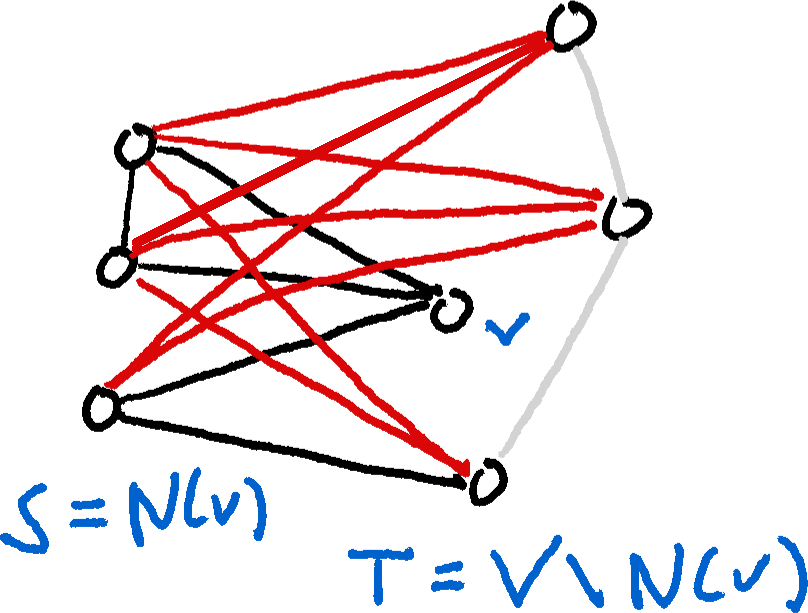
\includegraphics[width=0.6\textwidth]{graphics/L18_extremal_szemeredi/erdos_turan_proof.png}
        \caption[][0cm]{A figure of the construction of $H$ from $G$ in the Erd\H{o}s proof of Theorem \ref{thm:turan}. The black edges are edges that are kept, grey edges are removed, and red edges are added. The vertex $v$ and sets $S$ and $T$ are labelled in blue.}
        \label{fig:erdos_turan_proof}
    \end{figure}

    Now we construct a graph $H$ by taking $G$, deleting every edge inside of $T$, and adding every edge between $S$ and $T$. This construction is illustrated in Figure \ref{fig:erdos_turan_proof}.

    Since $G[S]$ is $(r-1)$-clique-free, adding a new neighbour to all of them cannot create an $r$-clique, so $H$ is still $r$-clique-free. It remains to see that it has at least as many edges as $G$.

    So consider the degree of any vertex $w$. If $w = v$, its degree didn't change, if $w \in S$, its degree can only have increased, and if $w \in T$ its new degree is $d_v$, which by assumption was maximum, so it again has not decreased. So since the degree of every vertex has increased or remained unchanged, we conclude that $\abs{E(H)} \geq \abs{E(G)}$.

    So we conclude that the maximal $r$-clique-free graphs must be ones which are unchanged by this process, and a moment's thought reveals that these must be precisely the complete multipartite graphs.\sidenote[][]{\begin{xca}Think for a moment.\end{xca}}
\end{proof}

We can actually employ the idea in this proof to answer a related question: If a triangle-free graph has very nearly $\ex(n; K_3)$ edges, will it be very close to being bipartite?\sidenote[][]{I first saw this proof in a summer school in Prague in 2022, and when the lecturer there introduced this proof he said that it was extremely nice, and if we ever taught a course on graph theory, we had to include it. So now, a year and a half later, I \emph{am} teaching a course on graph theory, and so I dug it up, found it is indeed very nice, and included it.} Results of this kind are called \emph{stability} results, since they answer questions of the type ``if you nudge the extremal object a bit, will it still look similar''.

\begin{theorem}[Simonovits 1968, Füredi 2015]
    Every triangle free graph with $\ex(n, K_3) - t$ edges may be made bipartite by removing $t$ edges.

    \begin{proof}
        Take $G = (V,E)$ to be such a graph, and as before, pick $v \in V$ to be a vertex of maximum degree. We set
        $$A = V \setminus N(v), \qquad B = N(v)$$
        and notice that due to triangle-freeness, there can be no edges internal to $B$.

        Let us consider the sum of the degrees of the vertices in $A$. On the one hand, we can compute
        \begin{align*}
            \sum_{w \in A} d_w &= 2e(A) + e(A,B)\\
            &= e(A) + \left(e(A) + e(A,B) + e(B)\right) = e(A) + e(G)\\
            &= \ex(n; K_3) - t + e(A).
        \end{align*}

        On the other hand, we have since $d_v$ is maximum, that
        \begin{align*}
            \sum_{w \in A} d_w \leq \abs{A}d_v = (n-d_v)d_v \leq \ex(n; K_3).
        \end{align*}
        Here, the final inequality follows from that $(n-d_v)d_v$ is precisely the number of edges of a complete bipartite graph with parts of size $d_v$ and $n-d_v$, which is certainly triangle free on $n$ vertices and thus has at most $\ex(n; K_3)$ edges.

        So we have seen that $\ex(n; K_3) \geq \ex(n; K_3) - t + e(A)$, so $e(A) \leq t$. So if we remove these at most $t$ edges, there will be no edges internal to either $A$ or $B$, and so $G$ will be bipartite.
    \end{proof}
\end{theorem}

\section{Szemerédi's regularity lemma and the triangle removal lemma}

As we explored in the exercises, the Szemerédi regularity lemma tells us that all large enough graphs look roughly like a random multipartite graph, so their structure can be summarized by a ``blueprint'' graph. Let us now see how we can use this result to see a sort of converse result to our previous result about nearly maximum triangle-free graphs.

In particular, the result we are going to show states that if you need to remove a large amount of edges to destroy every triangle in the graph, then the graph must in fact have contained a lot of triangles.

\begin{theorem}[Erd\H{o}s-Simonovits, 1983]\label{thm:triangle_removal}
    For every $\varepsilon > 0$ there is a $\delta > 0$ such that if $G$ is an $n$-vertex graph such that at least $\varepsilon n^2$ edges have to be removed from $G$ in order to make it triangle-free, then $G$ has at least $\delta n^3$ triangles.
\end{theorem}

Since the proof of this uses Szemerédi regularity, let us restate that theorem here as well, along with a crucial definition used in its statement:

\begin{definition}
    Let $G = (V,E)$ be a graph on $n$ vertices, and $A$ and $B$ two disjoint subsets of $V$. For any $\varepsilon > 0$, we say that the pair $(A,B)$ is \emph{$\varepsilon$-regular} if it holds for all $X \subseteq A, Y \subseteq B$ with $\abs{X} \geq \varepsilon\abs{A}$ and $\abs{Y} \geq \varepsilon\abs{B}$ that
    $$\abs{d(X,Y) - d(A,B)} \leq \varepsilon.$$
\end{definition}

\begin{theorem}[Szemerédi's regularity lemma]
    For every $\varepsilon > 0$ and $m \in \N$ there exists an $M \in \N$ such that for every graph $G = (V,E)$ on at least $M$ vertices and every $\delta \in [0,1]$, there exists
    \begin{enumerate}[label=\alph*)]
      \item a blueprint $R = ([k],E_R,w)$ whose minimum weight is at least $\delta$,
      \item a partition $V = V_0 \coprod V_1 \coprod \ldots \coprod V_k$,
      \item and a spanning subgraph $G'$ of $G$,
    \end{enumerate}
    such that
    \begin{enumerate}
      \item $m \leq k \leq M$,
      \item $0 \leq \abs{V_0} \leq \varepsilon\abs{V}$,\sidenote[][]{So notice in particular that $V_0$ may be empty.}
      \item $\abs{V_1} = \abs{V_2} = \ldots = \abs{V_k}$,
      \item for every $v \in V$
      $$d_{G'}(v) > d_G(v) - (\delta + \epsilon)\abs{V},$$
      where $d_{G'}$ and $d_G$ denote degrees in $G'$ and $G$ respectively,
      \item the graph $G'' = G'[V\setminus V_0]$ is multipartite with the sets $V_i$ as parts,\sidenote[][]{Which concretely just means that for every $i = 1,2,\ldots,k$, there are no edges internal to $V_i$ in $G'$, which you could alternatively phrase as that these sets are independent in $G'$.}
      \item and all of the pairs $(V_i, V_j)$ for $1 \leq i, j \leq k$ are $\varepsilon$-regular, and their density is $w(i \sim j)$ if $i \sim j$ is an edge of $R$, and otherwise there are no edges between them. 
    \end{enumerate}
\end{theorem}

\begin{remark}
    The graph $G''$ will be multipartite, and have at most $\frac{\delta + 3\varepsilon}{2}n^2$ edges fewer than the graph $G$ we started with.\sidenote[][]{Showing this was one of the exercises in the exercise session on this topic.}
\end{remark}

Let us now give an idea of a proof of the triangle removal lemma -- except we avoid the details of what the exact values of our $\varepsilon$s and $\delta$s will be. We don't need to know that, and it would be painful to keep track of in a lecture.\sidenote[][]{If you wish, try to flesh out the proof with all those details -- or just use Google to find a fully detailed proof.}

\begin{proof}[Proof sketch of Theorem \ref{thm:triangle_removal}]
    Suppose $G$ is a graph satisfying the hypotheses of the theorem, that is, it has $n$ vertices and you need to remove at least $\varepsilon n^2$ edges to make it triangle-free.

    Then we can pick some $\varepsilon_0$ and $\delta$ such that we, when we insert those into the regularity lemma, get a blueprint $R$ and a multipartite subgraph $G''$ of $G$ which has had less than $\epsilon n^2$ edges removed.

    Then, by our hypothesis, this $G''$ must contain a triangle, and since it is multipartite the vertices of this triangle must belong to three different parts $V_i, V_j, V_k$.

    Thus there has to be a triangle $\{i, j, k\}$ in the blueprint $R$, and the weight of each of the edges of this triangle has to be at least $\delta$. The intuition now is that $G''$ looks like a random multipartite graph with blueprint $R$, and in such a random multipartite graph we would expect to see
    $$w(i\sim j)w(i\sim k)w(k\sim j)n^3 \geq \delta^3 n^3$$
    triangles between the three parts.

    Now, we can of course not reason like that, because the graph $G$ is not actually random -- however, all the three pairs $(V_i, V_j)$, $(V_i, V_k)$ and $(V_j, V_k)$ are $\varepsilon_0$-regular, which essentially means that they can't behave too differently from the behaviour of a random graph. So applying the regularity property a few times,\sidenote[][0cm]{
        In particular, the following lemma comes in handy:
        \begin{lemma}
            Let $(A,B)$ be an $\varepsilon$-regular pair with density $d$ in a graph $G$. For any $a \in A$ and $Y \subseteq B$, let
            $$d_Y(a) = d_{G[Y\cup\{v\}]}(a),$$
            that is, $d_Y(v)$ is the number of neighbours of $a$ in $Y$.
            
            It holds that, if $\abs{Y} \geq \varepsilon\abs{B}$, we have
            $$\abs{\left\{a \in A \given d_Y(a) < (d - \varepsilon)\abs{Y}\right\}} < \varepsilon\abs{A}.$$

            That is, for any large enough subset $Y$ of $B$, nearly all vertices of $A$ have the expected number of neighbours in $Y$.
        \end{lemma}
    } we see that there is indeed a $\delta'$ such that $G''$, and thus also $G$, has at least $\delta' n^3$ triangles.
\end{proof}

\section{Exercises}


%\bibliography{references}
%\bibliographystyle{plainnat}

\end{document}
